\documentclass{beamer} 
%\title{text}
%\author{text}
%\date{date}

\usepackage{tikz}
\usetikzlibrary{mindmap,trees}
\usepackage{verbatim}
\usepackage{adjustbox}

\begin{document}
\begin{frame}
	\titlepage
\end{frame}

\begin{frame}{TITLU FRAME}

\begin{itemize}
	\item The body
	\pause
	\item ALt body
	\pause
	\item altu
\end{itemize}

\end{frame}

\begin{frame}
\begin{adjustbox}{max totalsize={.9\textwidth}{.7\textheight},center}
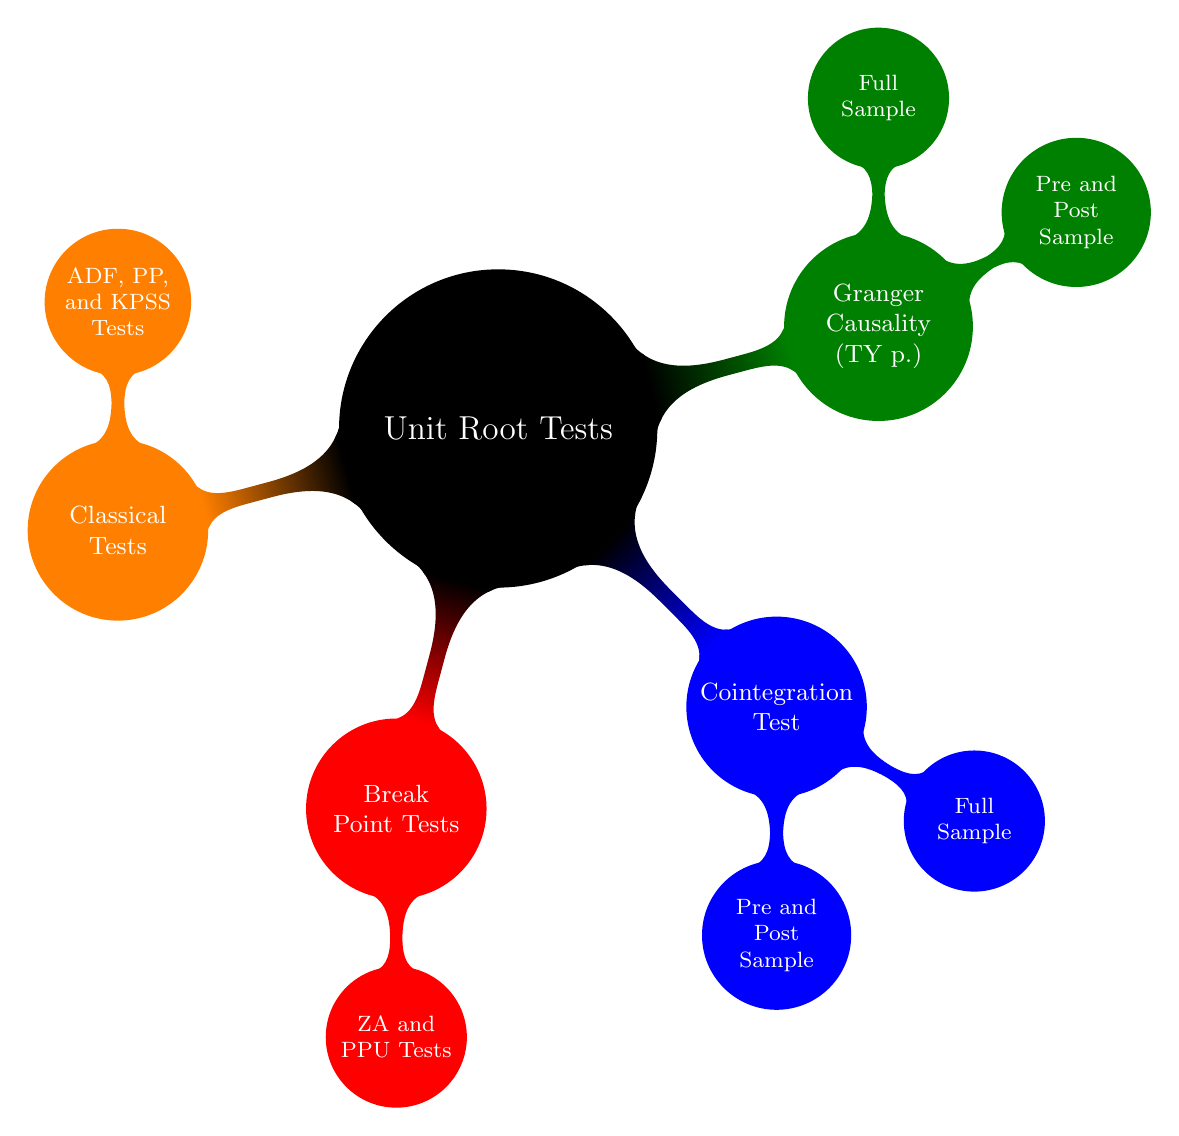
\begin{tikzpicture}
  \path[mindmap,concept color=black,text=white]
    node[concept] {Unit Root Tests}
    [clockwise from=15]
    child[concept color=green!50!black] {
      node[concept] {Granger Causality (TY p.)}
      [clockwise from=90]
      child { node[concept] {Full Sample}}
      child { node[concept] {Pre and Post Sample}}
    }  
    child[concept color=blue] {
      node[concept] {Cointegration Test}
      [clockwise from=-30]
      child { node[concept] {Full Sample} }
      child { node[concept] {Pre and Post Sample} }
    }
    child[concept color=red] { node[concept] {Break Point Tests} [clockwise from=-90] 
        child { node[concept] {ZA and PPU Tests}}}
    child[concept color=orange] { node[concept] {Classical Tests} [clockwise from=90] 
        child { node[concept] {ADF, PP, and KPSS Tests}}};
\end{tikzpicture}
\end{adjustbox}
\end{frame}
\end{document}

